\documentclass{article}
\usepackage{geometry}
\usepackage{graphicx}
\usepackage{amsmath}
\usepackage{amsfonts}
\usepackage{color}
\usepackage{listings}
\usepackage{float}
\geometry{a4paper,margin=1in}


\title{
\textbf{\begin{tabular}{c}Exercise 3: Threading, Tasking and\\ Real Time Synchronization\end{tabular}}}
\author{\Large
\begin{tabular}{l@{\hspace{2em}}r}Zachary \textsc{Vogel}&  Vidya \textsc{Karungaran}\end{tabular}
\\[1.5ex]
\begin{tabular}{l@{\hspace{2em}}r}ECEN 5623 & Timothy \textsc{Scherr}\end{tabular}}
\date{March 5th, 2016}

\begin{document}

\maketitle

\section*{Problem 1}
\subsection*{3 points of Priority Inheritance}
\begin{itemize}
    \item Lemma 6 is huge because it tells us that a job can be blocked at most 1 time per semaphore it uses. This is key because the blocking time for each semaphore must be bounded assuming no job has infinite execution. This overall leads to a job that has a finite upper bound on its blocking time.
    \item Lemma 9 is an essential point of the priority ceiling protocol because it states that there can never be transitive blocking with this protocol. Thus, a job at low priority will be immediately pushed to the highest priority of all jobs it could block for any given semaphore.
    \item Lemma 11 is interesting, stating that a higher priority job can be blocked by a lower priority one for at most the duration of one critical section of all of the lower priority tasks critical sections
\end{itemize}

\subsection*{Position on Linux Priority Inheritance}
Our group will be taking the opinion that Linux Priority Inheritance is a good thing, and can be extremely useful depending on the application. While Linus Torvalds seems to take the position that any priority inversion problem can be solved without Priority Inheritance, that is unrealistic in a development sense. The fact of the matter is that Priority Inheritance solves the problem of Priority Inversion. The main problem with Priority Inversion is that it gives a low priority task high priority. In Linux this might be bad because the low priority task could potentially write to locations where they shouldn't normally. That is overcome by running code in user space, and never giving high enough priority to a task so that it overwrites kernal space memory. The only other reason that Priority Inheritance is bad is because there are potentially other implementations that don't even require it. If one didn't use blocking then this would never happen, but that requires one to give each function a copy of the memory it works on which isn't efficient. It is generally possible to write code where Priority Inversion never happens, but that may require significant extra testing and work. By solving the problem with Priority Inheritance, we give a solution that, despite its drawbacks, can be made to work better and more easily than other solutions, which is what engineering is all about.

\subsection*{Does PI\_Futex Fix it?}
The PI\_Futex does prevent a high priority task from unbounded priority inversion in the user space. By implementing the PI\_Futexs largely the same as normal Futexs for the fast path, while not invoking any kernel calls for the short path, Ingo Molnar has made a safe implementation of Priority Inheritance locking. Similarly, the implementation for slow lock uses a minimal amount of kernel calls while looking up the priority of the highest waiting task. Overall, it seems like a very good implementation, but it isn't in the kernel. 


\section*{Problem 2}
\subsection*{Thread-Safe, and Reentrant}
Thread-safe functions are functions that only ever access shared data safely, this means multiple calls to this function at the same time won't have any negative effect. A reentrant function is one that can be interrupted or preempted and then called again safely without finishing execution of the original call.

\subsection*{Three Solutions}
The first method of accomplishing this is by only using stack variables,and not using global data or dynamic memory. To do this, every single function must be passed all of the data it needs and must return all of the data it processes probably in the form of pointers to structures. It is often cumbersome to do this, and could potentially lead to over-sized structures getting passed in unnecessarily. The real issue is that one must copy all of the data every time a function call is made, which is extremely inefficient.
Since the variables are declared locally to a function, it is thread safe as each thread working on the function will have a local copy of the variable unlike a global variable declaration which would result in race condition. But the threads must be executed in order (with proper priority assigned to each thread) so that we do not face issues with data forwarding. 

The problem with the second method would be synchronization between threads. If the threads need to share data, then a shared memory has to be used again with semaphores and mutexs. Care must be taken in assigning priorities to each thread. Transferring data from global memory for the computation will result in lesser throughput due to high latency. Since the data is thread indexed, one is either going to have to make many copies of the same memory or implement proper locking mechanisms to prevent shared memory errors.

The final method of accomplishing this is to use shared memory global data, but to use locking mechanisms to synchronize access. This method can be implemented with semaphores and mutexs like the POSIX standard ones. The idea is to allow only one thread to work on the shared memory at a time by implementing a type of counter (note mutexs and semaphores aren't necessarily implemented as counters). If that counter is zero then that thread must wait, if it is one or more than it can execute on the shared memory. It does have drawbacks, like unbounded priority inversion or unbounded blocking, but these can generally be overcome fixed with proper coding techniques.

\subsection*{An Implementation with Pthreads}
Here is a screencapture of our implementation of code to randomly generate data and a timestamp in one thread and then print it out safely in another. A makefile is included in the folder PR\_2 that allows one to build and clean this.
\begin{figure}[H]
    \centering
    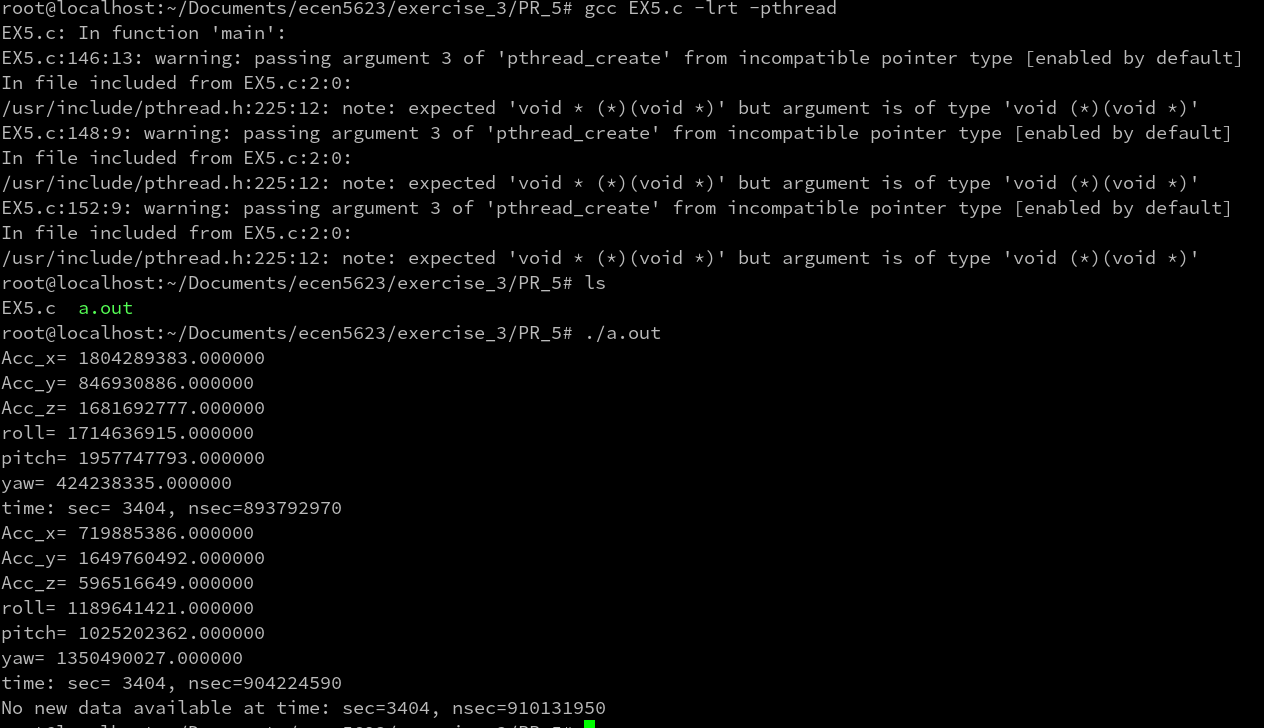
\includegraphics[width=0.9\textwidth]{execution.png}
    \caption{Code that writes and reads some data safely}
\end{figure}
\section*{Problem 3}
\subsection*{Deadlock}
Deadlock is what happens when threads are looking for more than one shared piece of memory. If one thread takes shared memory A, and another thread takes shared memory B, then the first thread asks for shared memory B and the second thread asks for shared memory A execution of each thread will stop indefinitely. One solution to this, known as random backoff, is to give up the resource a thread owns when it tries and fails to get the other resource. Then, wait a psuedo-random amount of time, and try to grab each resource again. In that period of wait time the other thread will hopefully get both pieces of memory and finish with shared memory. This is what we implemented on the deadlock code given to us for the problem.
\subsection*{Priority Inversion}
Priority Inversion is another effect of having multiple priority level tasks/services and shared resources. When a low priority and high priority task both share data, the low priority task might end up blocking the high priority task. Basically, the low priority task will have the shared memory and be executing on it, the high priority task will need to wait for that to finish, but a medium priority task could preempt the low priority task and force the high priority task to wait for many lower priority tasks to finish while waiting for the shared memory. This kind of inversion was demonstrated by the code given to us and can be seen running below.

\subsection*{Linux RT Preempt Patch}
The Linux real-time preempt patch is a patch that exists to fix the issues of Linux only being able to meat soft real-time deadlines. This patch attempts to address priority inversion by creating priority inheritance. This means that when a high priority thread is blocked because a low priority thread is using shared memory the low priority thread will inherit the high priority thread's priority for the duration of its use of shared memory. Thus, the low priority thread can no longer be preempted by medium priority ones.

This method does address the unbounded priority inversion because the high priority thread can no longer be stuck behind infinite medium priority threads. With this technique, the high priority thread is blocked for only the duration the low priority thread is using shared memory. The downside of this technique is that the low priority thread gets high priority for much of its execution, which isn't necessarily desirable. If the high priority thread is using the shared memory of an even higher priority thread, the low priority thread could even be pushed all the way up to that higher priority. A developer might pursue a different implementation where the low priority thread simply never executes its critical section if it would preempt in any way the higher priority thread. A system like that might limit blocking time for high priority tasks, but would likely be harder to implement. That is where something like priority inversion becomes useful. While it doesn't address the entire issue of priority inversion it does address the problem of unbounded priority inversion.

The question of switching to a RTOS because of the problems of priority inversion in Linux is an interesting one. A RTOS might address the issues of priority inversion a lot better than Linux does even with the preempt patch, but probably does not come with the same community and sheer amount of code that has gone into Linux. For projects from companies where much of the code will be written from scratch anyway, a RTOS will probably be the better solution because it is more specifically tailored to real-time applications than Linux will ever be. On the other hand, Linux does provide a lot of non-embedded system tools that might be extraordinarily useful for some applications.
\subsection*{Deadlock and PI Code Running}
Here is the proof of execution of our code to fix the deadlock with a random backoff scheme. There is a makefile in the PR\_2/new folder which will allow one to run this code after running ./deadlock as an executable.
\begin{figure}[H]
    \centering
    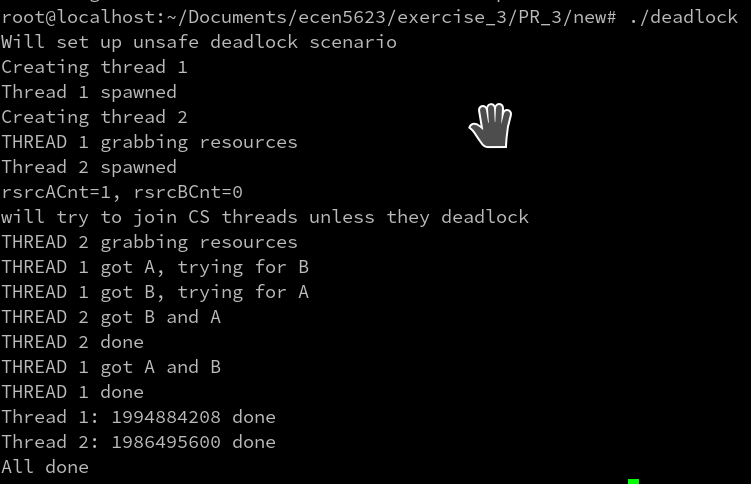
\includegraphics[width=0.8\textwidth]{deadlock_fixed.png}
    \caption{Here is the fixed deadlock code executing}
\end{figure}

Additionally, we built and ran the original code, located in PR\_2/old. Here are screenshots of that running on the DE1.
\begin{figure}[H]
    \centering
    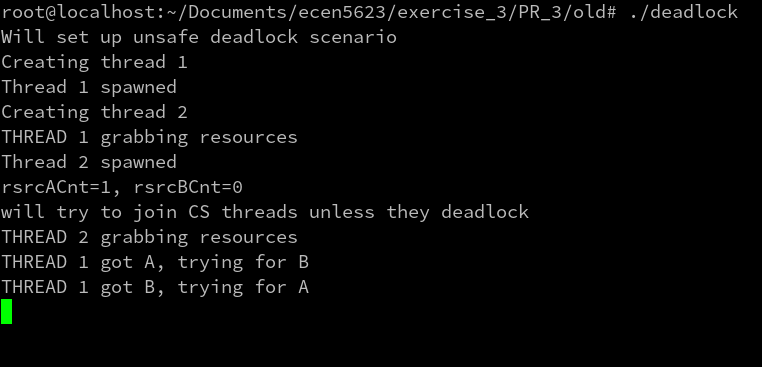
\includegraphics[width=0.8\textwidth]{deadlock.png}
    \caption{original deadlock code deadlocking}
\end{figure}
\begin{figure}[H]
    \centering
    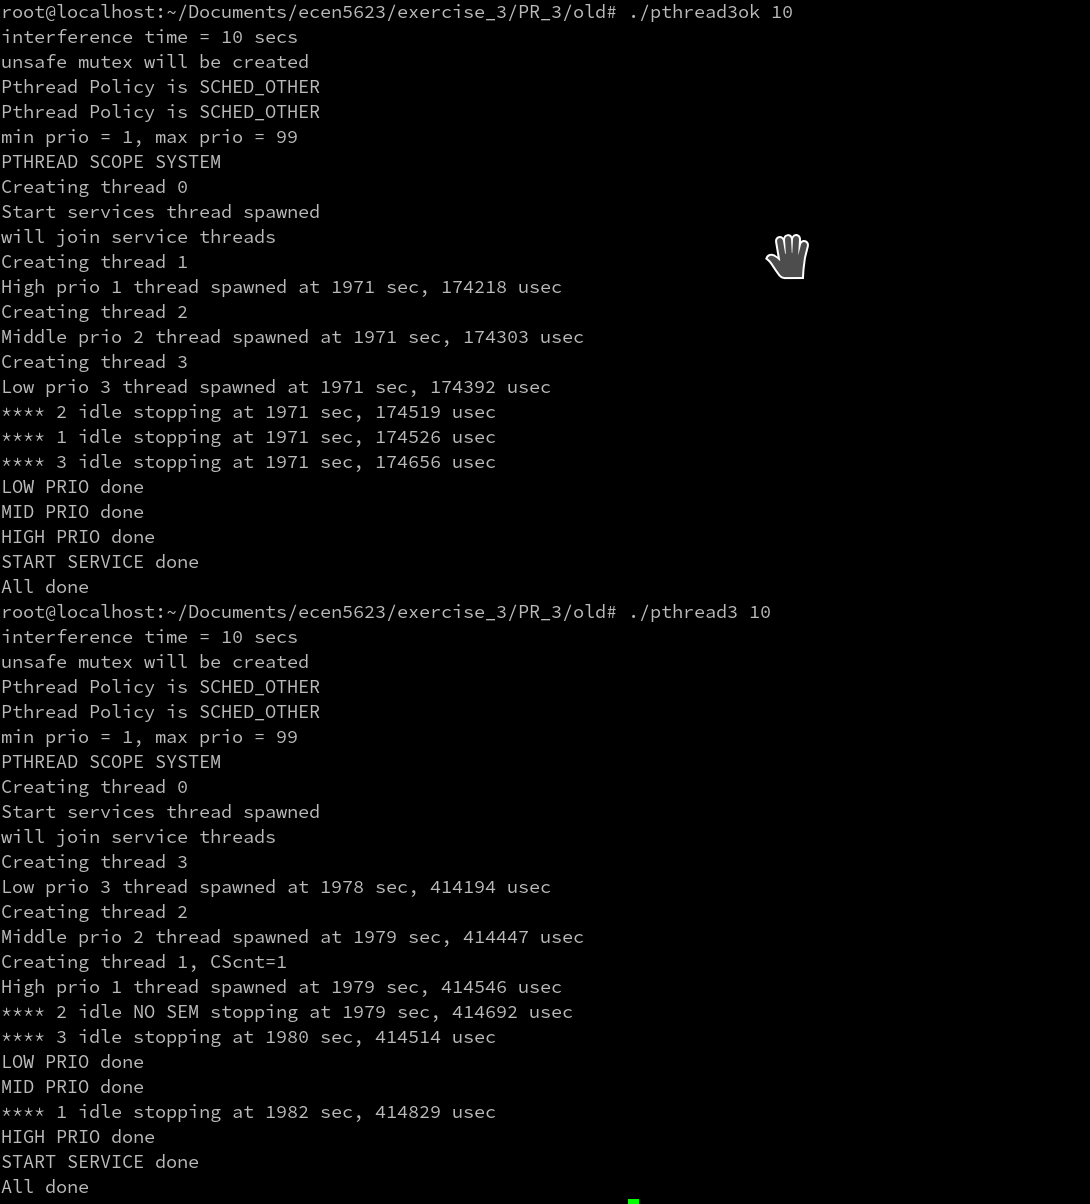
\includegraphics[width=0.8\textwidth]{pthread_ok.png}
    \caption{Both sets of pthread code executing}
\end{figure}    


\section*{Problem 4}
\subsection*{Message Queues and Global Memory Sharing}
Message queues prevent the problem of unbounded priority inversion as the enqueue and dequeue operations are thread safe. It services messages in the order of priority and guarantees message delivery in a timely fashion. Therefore a low priority task cannot be preempted by a medium priority task. So the higher priority task waiting on the lower priority task  waits for deterministic amount of time thus avoiding unbounded priority inversion.
\subsection*{Fixing and Running Old Code}
We never ended up having time to fix the heap\_mq.c implementation properly as can be seen by trying to compile and run it. It works kind of, but ends up crashing. Additionally, neither of these sets of code ran on the DE1 board because the mqueue library was not implemented as can be seen in figure 5. A makefile is included which will build this code properly on both a normal linux install and the DE1, but mqueue functions aren't actually implemented on Lubuntu for the DE1. This was checked using the perror, error message.

\begin{figure}[H]
    \centering
    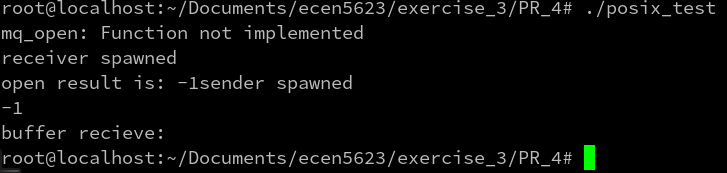
\includegraphics[width=0.8\textwidth]{not_implemented.png}
    \caption{Functions are declared but not implemented on DE1}
\end{figure}
\begin{figure}[H]
    \centering
    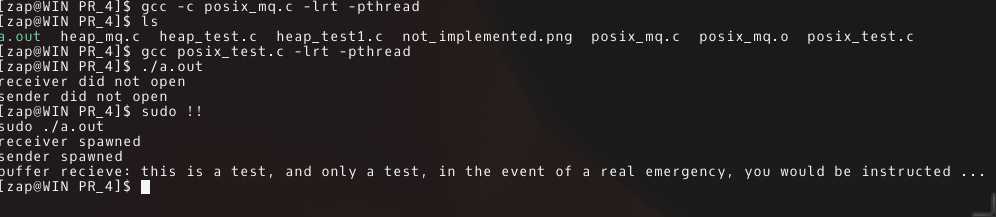
\includegraphics[width=0.8\textwidth]{posix_save.png}
    \caption{The posix message queue compiling and running on a Linux install}
\end{figure}
\begin{figure}[H]
    \centering
    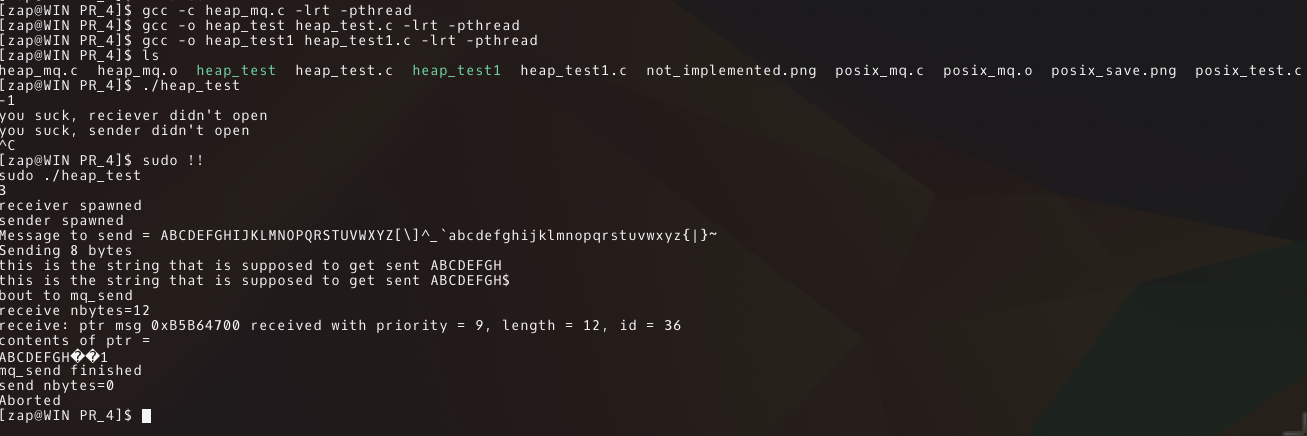
\includegraphics[width=0.8\textwidth]{heap_save.png}
    \caption{The heap message queue compiling and failing to run properly on a Linux install}
\end{figure}
\section*{Problem 5}
\subsection*{Linux Watchdog Timer}
The Linux Watchdog Timer is used by the Linux Watchdog Daemon to act as stand-alone system monitor. The watchdog daemon for Linux can be configured to periodically run  several basic tests to verify that the system is functioning properly.It opens /dev/watchdog, and keeps writing to it every minute or so to keep the kernel from resetting.When a deadlock occurs, then the watchdog will not be serviced and the system will be reset, thus coming out of deadlock situation. But the system might get into a live lock, a situation where the system gets into a deadlock after coming out of reset.
\subsection*{Problem 2 Code Adaptation}
Here is the adaption showing a mutex\_timedlock for sharing data. It prints that no new data is ready after 10 seconds of waiting and exits when it finally does get the data.
\begin{figure}[H]
    \centering
    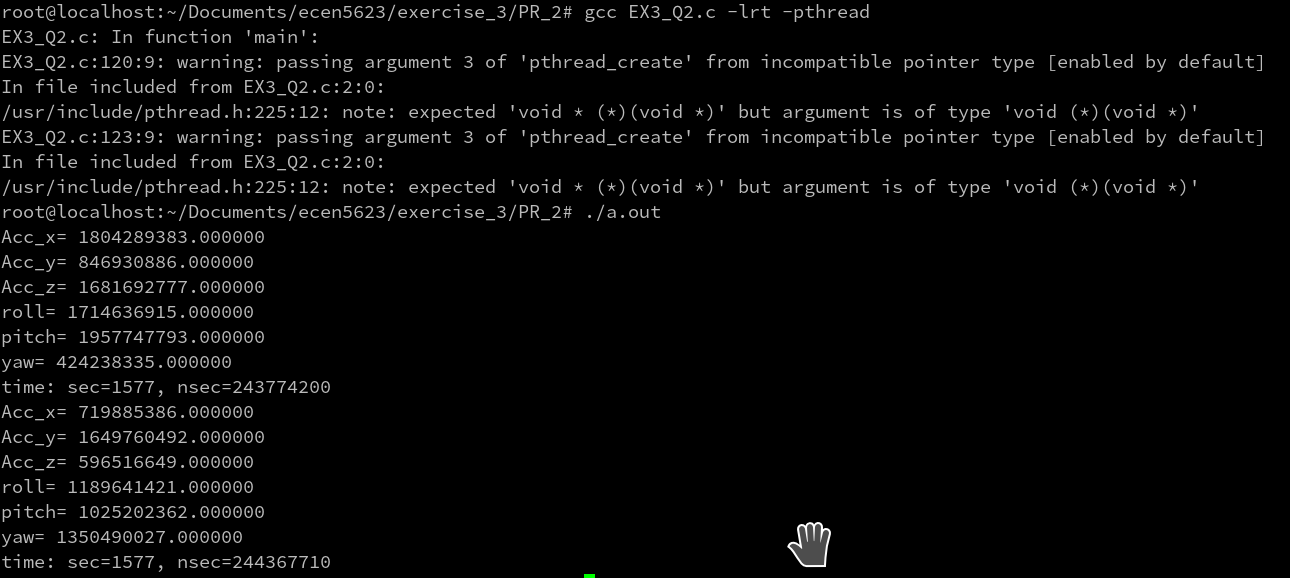
\includegraphics[width=0.8\textwidth]{run.png}
    \caption{Code for problem 5 running on the DE1}
\end{figure}

\end{document}

